\section{The Relative Two-Body Problem}\label{sec:Relative2BP}
This investigation treats the behavior of spacecraft in heliocentric space, specifically when they
are far from planets and moons, as a relative 2-body Problem, governed by a single gravitational
force. This section provides a brief overview of key aspects of relative 2BP dynamics, Keplerian
orbital elements, and Kepler's Equation. For a more comprehensive derivation of the 2BP, refer to
Chapters 1 and 2 of Vallado's \emph{Fundamentals of Astrodynamics and
Applications}\cite{Vallado:2013}. Additionally, Canales highlights the background information
relevant to understanding the transfer methodologies presented in this
analysis\cite{Canales:2021b}.

\subsection{Equations of Motion}
The relative 2BP involves two point masses, for example, a primary body and a spacecraft, that
exert gravitational forces on each other. Since external forces are not acting on the system, the
center of mass of these two bodies moves at a constant velocity and serves as the origin for an
inertial coordinate frame. In the inertial frame, the gravitational force that the primary body
exerts on the spacecraft, denoted as $\Fbar_{g_{P\rightarrow s/c}}$, is expressed as:
\begin{equation}
    \Fbar_{g_{P\rightarrow s/c}}=-\frac{Gm_{P}m_{s/c}}{r_{P\rightarrow s/c}^{3}}\rbar_{P\rightarrow s/c},
    \label{eq:gravity}
\end{equation}
where $G$ is the universal gravitational constant (6.67384x10$^{-20}$ kN*km$^{2}$/kg$^{2}$),
$m_{P}$ and $m_{S}$ are the masses of the primary and secondary body, e.g., a spacecraft,
respectively, $r_{P\rightarrow s/c}$ is the distance from the primary body to the spacecraft, and
$\rbar_{P\rightarrow s/c}=\rbar_{s/c}-\rbar_{P}$ is the relative position vector from the primary
body to the spacecraft in the inertial frame, as illustrated in \cref{fig:2BP}.

\begin{figure}[H]
    \centering
    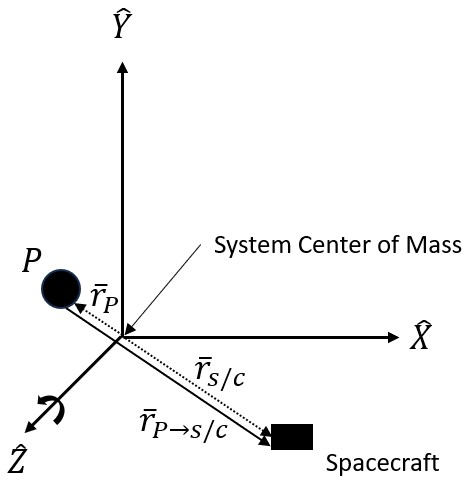
\includegraphics[width=0.5\textwidth]{figures/TBP.jpg}
    \caption{Two-body problem in a barycentric inertial frame.}
    \label{fig:2BP}
\end{figure}

Within the relative inertial frame, the 2BP equations of motion are derived in both vector and
scalar forms\cite{Vallado:2013,Canales:2021b}. Assuming that the secondary mass is negligible
compared to the mass of the primary body, in the $\{\Xhat,\Yhat\Zhat\}$ inertial frame:
\begin{equation}
    \rbarddot_{P\rightarrow s/c}=-\frac{\mu_{2BP}}{r_{P\rightarrow s/c}^{3}}\rbar_{P\rightarrow s/c},
    \label{eq:TBPEoM}
\end{equation}
\vspace{1mm}
\begin{equation}
    \Xddot=-\frac{\mu_{2BP}}{r_{P\rightarrow s/c}^{3}}(X_{s/c}-X_{P}),
    \label{eq:TBPEoMX}
\end{equation}
\vspace{1mm}
\begin{equation}
    \Yddot=-\frac{\mu_{2BP}}{r_{P\rightarrow s/c}^{3}}(Y_{s/c}-Y_{P}),
    \label{eq:TBPEoMY}
\end{equation}
\vspace{1mm}
\begin{equation}
    \Zddot=-\frac{\mu_{2BP}}{r_{P\rightarrow s/c}^{3}}(Z_{s/c}-Z_{P}),
    \label{eq:TBPEoMZ}
\end{equation}
where $\rbarddot_{P\rightarrow s/c}$ is the inertial acceleration vector of the spacecraft relative
to the primary body, $\Xddot$, $\Yddot$, and $\Zddot$ are the scalar components of that
acceleration, and $\mu_{2BP}=Gm_{P}$. These equations of motion are employed to describe spacecraft
behavior in heliocentric space in this investigation.

\subsection{Conic Sections}
Instead of relying on numerical propagation of the nonlinear equations of motion, spacecraft
behavior in the relative 2BP is effectively represented analytically through conic sections. Two
essential constants characterize conic orbits: specific angular momentum $\ambar$ and specific
mechanical energy $\mathcal{E}$:
\begin{equation}
    \ambar=\rbar_{P\rightarrow s/c}\times\rbardot_{P\rightarrow s/c},
    \label{eq:angularmomentum}
\end{equation}
\vspace{1mm}
\begin{equation}
    \mathcal{E}=\frac{v_{P\rightarrow s/c}^{2}}{2}-\frac{\mu_{2BP}}{r_{P\rightarrow s/c}},
    \label{eq:energy}
\end{equation}
where $v_{P\rightarrow s/c}=||\rbardot_{P\rightarrow s/c}||_{2}$ is the spacecraft velocity in the
inertial frame relative to the primary body. Kepler's first law, asserting that orbital motion is
conic, provides the trajectory equation for the 2BP:
\begin{equation}
    r_{P\rightarrow s/c}=\frac{a(1-e^{2})}{1+e\cos(\theta)},
    \label{eq:trajectory}
\end{equation}
where $a$ represents the orbit semimajor axis, $e$ is the orbit eccentricity, and $\theta$ denotes
the orbit true anomaly. \cref{eq:trajectory} is also employed to compute the periapsis and apoapsis
distances, $r_{p}$ and $r_{a}$ respectively:
\begin{equation}
    r_{p}=a(1-e),
    \label{eq:periapsis}
\end{equation}
\begin{equation}
    r_{a}=a(1+e).
    \label{eq:apoapsis}
\end{equation}
The eccentricity also signifies the type of conic section:
\begin{itemize}
    \item   $0<e<1$: Elliptical orbit ($e=0$ represents a circular orbit).
    \item   $e=1$: Parabola.
    \item   $e>1$: Hyperbola.
\end{itemize}
Similarly, Kepler's third law provides the orbit period $\mathbb{P}$ and, consequently, the mean
motion:
\begin{equation}
    \mathbb{P}=2\pi\sqrt{\frac{a^{3}}{\mu_{2BP}}},
    \label{eq:period}
\end{equation}
\vspace{1mm}
\begin{equation}
    n=\frac{2\pi}{\mathbb{P}}=\sqrt{\frac{\mu_{2BP}}{a^{3}}}.
    \label{eq:meanmotion}
\end{equation}
This investigation focuses on arc segments of circles and ellipses in the 2BP with $0\leq e<1$.

\subsection{Keplerian Orbital Elements}
Instead of specifying the six-dimensional state of a spacecraft in a relative 2BP elliptical orbit
via Cartesian coordinates, six orbital elements are employed to articulate the size, shape,
orientation, and current location along the orbit. In addition to the semimajor axis $a$ and
eccentricity $e$, that were introduced earlier and describe the size and shape of the ellipse,
three angles characterize the orientation of the orbit with respect to an inertial frame, as
illustrated in \cref{fig:orbitalElements}:
\begin{itemize}
    \item \textbf{Inclination} $i$ signifies the tilt of the orbital plane relative to the inertial
    $\Xhat_{Ec}\Yhat_{Ec}$-plane.
    \item \textbf{Right ascension of the ascending node} (RAAN) $\Omega$ denotes the angle between
    the $\Xhat_{Ec}$-axis and the ascending node, where the orbit crosses the
    $\Xhat_{Ec}\Yhat_{Ec}$-plane in the positive $\Zhat_{Ec}$ direction.
    \item \textbf{Argument of periapsis} $\omega$ is the angle between the ascending node and the
    periapsis.
\end{itemize}
Finally, the true anomaly $\theta$ defines the spacecraft position relative to the orbit periapsis.
\cref{tab:orbitValues} provides the gravitational constants and some relevant orbital values for
the two-body systems employed in this investigation.

\begin{figure}[H]
    \centering
    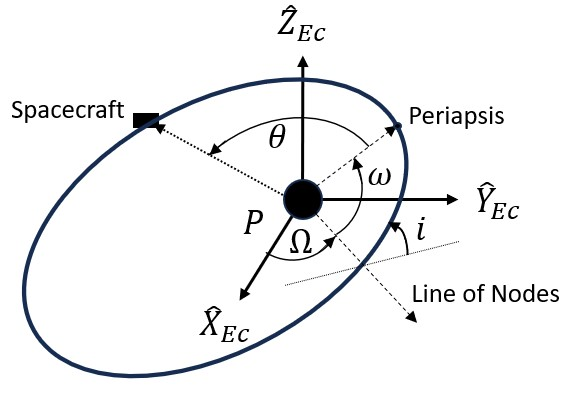
\includegraphics[width=0.5\textwidth]{figures/OrbitalElements.jpg}
    \caption{Orientation and location along an orbit in an inertial frame utilizing Keplerian orbital elements.}
    \label{fig:orbitalElements}
\end{figure}

\begin{table}[H]
    \centering
    \caption{Orbital values of relevant 2BP systems.}
    \begin{tabular}{|c|c|c|c|c|c|}
        \hline
        \textbf{Body}   &   \boldmath$\mu_{2BP}$ [\textbf{km}\boldmath$^{3}/$\textbf{s}\boldmath$^{2}$] &   \boldmath$a$ \textbf{[km]}  &   \boldmath$\mathbb{P}$ \textbf{[d]}  &   \boldmath$e$            &   \boldmath$i$ \textbf{[deg]} \\  \hline
        Sun             &   $1.32712\times10^{11}$                                                      &   -                           &   -                                   &   -                       &   -                           \\  \hline
        Earth           &   $398600$                                                                    &   $1.49598\times10^{8}$       &   $365.257$                           &   $1.67359\times10^{-2}$  &   $1.70780\times10^{-5}$      \\  \hline
        Moon            &   $4902.80$                                                                   &   $384748$                    &   $27.4892$                           &   $5.55455\times10^{-2}$  &   $5.15665$                   \\  \hline
        Mars            &   $42828.4$                                                                   &   $2.27941\times10^{8}$       &   $686.979$                           &   $9.34015\times10^{-2}$  &   $1.84971$                   \\  \hline
    \end{tabular}
    \label{tab:orbitValues}
\end{table}

\subsubsection{Cartesian state to Keplerian orbital elements}
While Keplerian orbital elements have their benefits, when transitioning between models and
coordinate frames, it is convenient to be able to convert between these elements and Cartesian
coordinates. To do so, starting from a Cartesian state, the inclination is calculated from the
angular momentum:
\begin{equation}
    i=\arccos(\frac{h_{Z}}{||\ambar||}).
    \label{eq:inclination}
\end{equation}
From the node vector $\nbar$:
\begin{equation}
    \nbar=\Zhat_{Ec}\times\ambar,
    \label{eq:nodes}
\end{equation}
the RAAN becomes:
\begin{equation}
    \Omega=\begin{cases}\arccos(\frac{n_{X}}{||\nbar||})&n_{Y}\geq0\cr2\pi-\arccos(\frac{n_{X}}{||\nbar||})&n_{Y}<0\end{cases}.
    \label{RAAN}
\end{equation}
The eccentricity vector $\ebar$ is also calculated from the angular momentum:
\begin{equation}
    \ebar=\frac{\rbardot_{P\rightarrow s/c}\times\ambar}{\mu_{2BP}}-\frac{\rbar_{P\rightarrow s/c}}{r_{P\rightarrow s/c}},
    \label{eq:eccentricityvector}
\end{equation}
and
\begin{equation}
    e=||\ebar||.
    \label{eq:eccentricity}
\end{equation}
The remaining three orbital elements are calculated as follows:
\begin{equation}
    a=\frac{||\ambar||}{\mu_{2BP}(1-e^{2})},
    \label{eq:semimajoraxis}
\end{equation}
\vspace{1mm}
\begin{equation}
    \omega=\begin{cases}\arccos(\frac{\nbar\cdot\ebar}{||\nbar||e})&e_{Z}\geq0\cr2\pi-\arccos(\frac{\nbar\cdot\ebar}{||\nbar||e})&e_{Z}<0\end{cases},
    \label{eq:argumentofperiapsis}
\end{equation}
and
\begin{equation}
    \theta=\begin{cases}\arccos(\frac{\ebar\cdot\rbar_{P\rightarrow s/c}}{er_{P\rightarrow s/c}})&v_{r}\geq0\cr2\pi-\arccos(\frac{\ebar\cdot\rbar_{P\rightarrow s/c}}{er_{P\rightarrow s/c}})&v_{r}<0\end{cases},
    \label{eq:trueanomaly}
\end{equation}
where
\begin{equation}
    v_{r}=\frac{\rbardot_{P\rightarrow s/c}\cdot\rbar_{P\rightarrow s/c}}{r_{P\rightarrow s/c}}.
    \label{eq:radialvelocity}
\end{equation}
These six elements define the Keplerian orbit as well as the specific state along that orbit.


\subsubsection{Keplerian orbital elements to Cartesian state}
Similarly, the Cartesian state vector can be obtained from the Keplerian orbital elements. First,
the eccentric anomaly $E$ is needed, the angle made by the eccentricity vector pointing to
periapsis and the vector from the center of the ellipse to the point directly above the spacecraft
location (perpendicular to the eccentricity vector) on an auxiliary circle drawn tangent to the
ellipse. The eccentric anomaly and the auxiliary circle are illustrated in \cref{fig:auxCircle},
along with the eccentricity vector and semimajor axis. The eccentric anomaly is related to the true
anomaly,
\begin{equation}
    E=\arctan(\frac{\sqrt{1-e^{2}}\sin(\theta)}{e+\cos(\theta)}),
    \label{eq:eccentricanomaly}
\end{equation}
that is then utilized to calculate the distance from the primary:
\begin{equation}
    r_{P\rightarrow s/c}=a(1-e\cos(E)).
    \label{eq:circularradius}
\end{equation}
These values lead to the position and velocity magnitude vectors:
\begin{equation}
    \rbar_{0}=\begin{bmatrix}r_{P\rightarrow s/c}\cos(\theta)\cr r_{P\rightarrow s/c}\sin(\theta)\cr0\end{bmatrix},
    \label{eq:circularpositionvector}
\end{equation}
\vspace{1mm}
\begin{equation}
    \rbardot_{0}=\sqrt{\frac{\mu_{2BP}a}{r_{P\rightarrow s/c}}}\begin{bmatrix}-\sin(E)\cr\sqrt{1-e^{2}}\cos(E)\cr0\end{bmatrix}.
    \label{eq:circularvelocityvector}
\end{equation}
The position and velocity vectors need to be rotated relative to the inertial frame axes according
to the inclination, RAAN, and argument of periapsis:
\begin{equation}
    C=\begin{bmatrix}\cos(\Omega)\cos(\omega)-\cos(i)\sin(\Omega)\sin(\omega)&-\cos(\Omega)\sin(\omega)-\cos(i)\sin(\Omega)\cos(\omega)&0\cr\sin(\Omega)\cos(\omega)+\cos(i)\cos(\Omega)\sin(\omega)&-\sin(\Omega)\sin(omega)+\cos(i)\cos(\Omega)\cos(\omega)&0\cr\sin(i)\sin(\omega)&\sin(i)\cos(\omega)&0\end{bmatrix},
    \label{eq:elementrotation}
\end{equation}
\vspace{1mm}
\begin{equation}
    \rbar_{P\rightarrow s/c}=C\rbar_{0},
    \label{eq:positionvector}
\end{equation}
\begin{equation}
    \rbardot_{P\rightarrow s/c}=C\rbardot_{0}.
    \label{eq:velocityvector}
\end{equation}
Finally, $\rbar_{P\rightarrow s/c}$ and $\rbardot_{P\rightarrow s/c}$ provide the six-dimensional
relative state in Cartesian coordinates.

\subsection{Kepler's Equation}
If the difference in true anomaly between two points on an orbit is known, Kepler's equation
becomes a valuable tool for calculating the time-of-flight between the two points. The mean anomaly
$M$ serves as a measure of the traversal of the orbit past periapsis with respect to time:
\begin{equation}
    M=\frac{2\pi(t-t_{p})}{\mathbb{P}},
    \label{eq:meananomaly}
\end{equation}
where $(t-t_{p})$ represents the time since periapsis. Kepler's equation then establishes a
connection between the mean and eccentric anomalies, thereby linking the eccentric anomaly to time:
\begin{equation}
    M=E-e\sin(E).
    \label{eq:Keplersequation}
\end{equation}
To determine eccentric anomalies given corresponding true anomalies, employ
\cref{eq:eccentricanomaly}, and subsequently, with Kepler's equation (\cref{eq:Keplersequation}),
convert them to mean anomalies. The difference in mean anomalies with \cref{eq:meananomaly}
provides the time-of-flight between the two points along the orbit.

\begin{figure}[H]
    \centering
    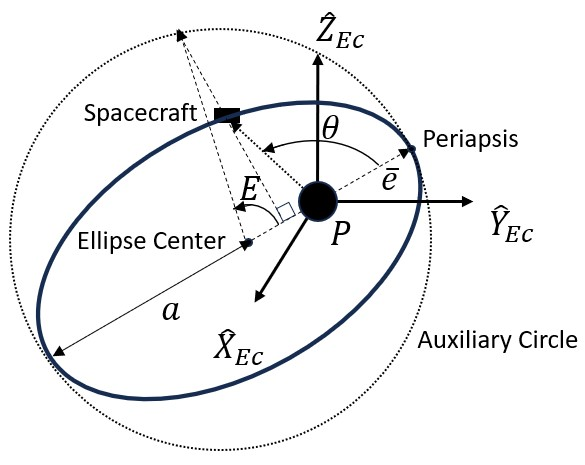
\includegraphics[width=0.5\textwidth]{figures/AuxCircle.jpg}
    \caption{Definition of eccentric anomaly and the auxiliary circle.}
    \label{fig:auxCircle}
\end{figure}
